\chapter{Square cylinder}
\section{Recirculation length}
\begin{table}[H]
	\centering
	\begin{tabular}{ |c|c|c| }
		\hline
		Re & Reference & Calculated \\ \hline
		1 & -0.0096 & 0.1067 \\ \hline
		3 & 0.1012 & 0.1865 \\ \hline
		5 & 0.212 & 0.2650 \\ \hline
		10 & 0.489 & 0.4474 \\ \hline
		30 & 1.597 & 1.4971 \\ \hline
		50 & 2.705 & 2.7702 \\ \hline
	\end{tabular}
\caption[Comparison of the recirculation length (Reference value vs. Calculated value)]{Comparison of the recirculation length (Reference value vs. Calculated value) \cite{Breuer2000}}
\end{table}

\section{Horizontal velocity}
\begin{figure}[H]
	\begin{subfigure}{\textwidth}
		\centering
		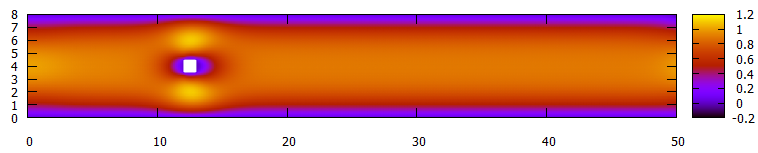
\includegraphics[width=.8\linewidth]{Square/totu1}
		\caption{$Re=1$}
	\end{subfigure}
	\begin{subfigure}{\textwidth}
		\centering
		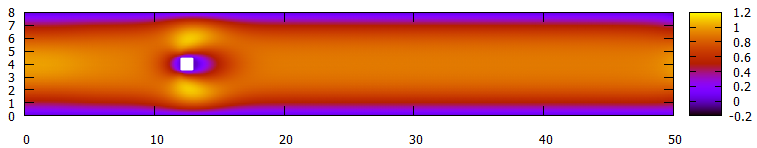
\includegraphics[width=.8\linewidth]{Square/totu3}
		\caption{$Re=3$}
	\end{subfigure}
	\begin{subfigure}{\textwidth}
		\centering
		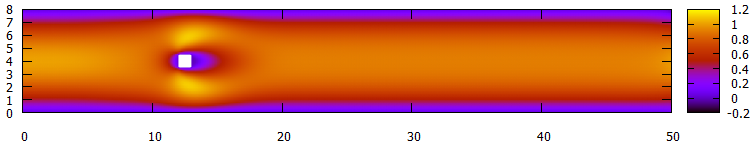
\includegraphics[width=.8\linewidth]{Square/totu5}
		\caption{$Re=5$}
	\end{subfigure}
	\begin{subfigure}{\textwidth}
		\centering
		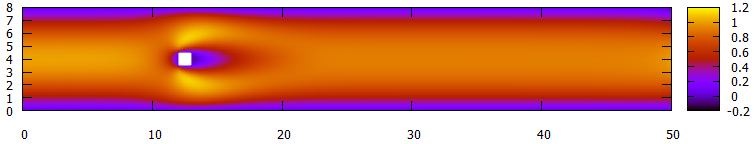
\includegraphics[width=.8\linewidth]{Square/totu10}
		\caption{$Re=10$}
	\end{subfigure}
	\begin{subfigure}{\textwidth}
		\centering
		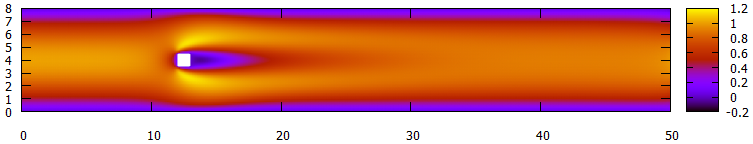
\includegraphics[width=.8\linewidth]{Square/totu30}
		\caption{$Re=30$}
	\end{subfigure}
	\begin{subfigure}{\textwidth}
		\centering
		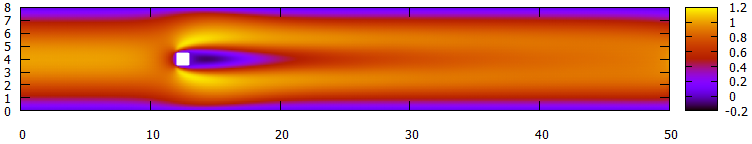
\includegraphics[width=.8\linewidth]{Square/totu50}
		\caption{$Re=50$}
	\end{subfigure}
\caption{Horizontal velocity in the channel}
\end{figure}

\section{Vertical velocity}
\begin{figure}[H]
	\begin{subfigure}{\textwidth}
		\centering
		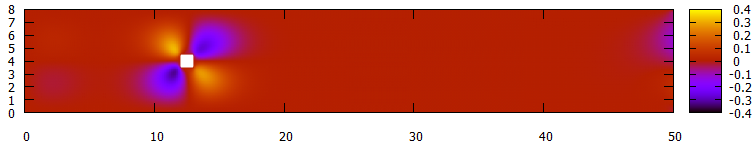
\includegraphics[width=.8\linewidth]{Square/totv1}
		\caption{$Re=1$}
	\end{subfigure}
	\begin{subfigure}{\textwidth}
		\centering
		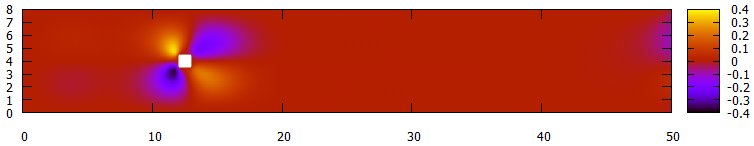
\includegraphics[width=.8\linewidth]{Square/totv3}
		\caption{$Re=3$}
	\end{subfigure}
	\begin{subfigure}{\textwidth}
		\centering
		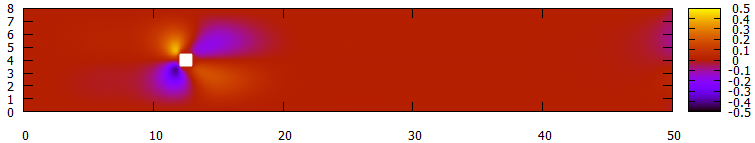
\includegraphics[width=.8\linewidth]{Square/totv5}
		\caption{$Re=5$}
	\end{subfigure}
	\begin{subfigure}{\textwidth}
		\centering
		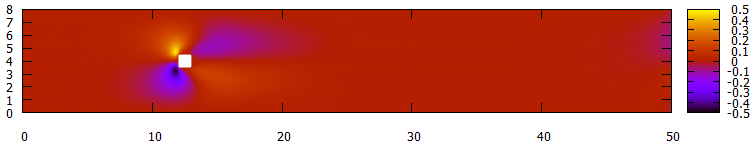
\includegraphics[width=.8\linewidth]{Square/totv10}
		\caption{$Re=10$}
	\end{subfigure}
	\begin{subfigure}{\textwidth}
		\centering
		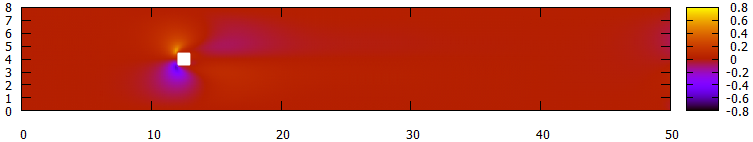
\includegraphics[width=.8\linewidth]{Square/totv30}
		\caption{$Re=30$}
	\end{subfigure}
	\begin{subfigure}{\textwidth}
		\centering
		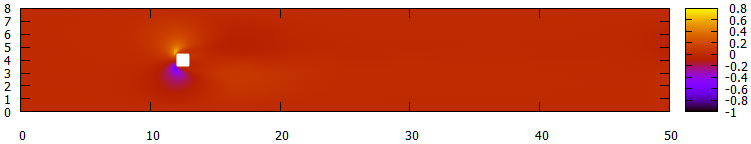
\includegraphics[width=.8\linewidth]{Square/totv50}
		\caption{$Re=50$}
	\end{subfigure}
	\caption{Vertical velocity in the channel}
\end{figure}